%%%%%%%%%%%%%%%%%%%%%%%%%%%%%%%%%%%%%%%%%%%%%%%%%%%%%%%%%%%%%%%%%%%%%%%%%%%%%%%
\section{Future Work}
%%%%%%%%%%%%%%%%%%%%%%%%%%%%%%%%%%%%%%%%%%%%%%%%%%%%%%%%%%%%%%%%%%%%%%%%%%%%%%%

{\tt abelfunctions} provides a collection of tools for computing on
Riemann surfaces. Although a few more features need to be added most of
the package's functionality is ready to be used to solve problems. In
this chapter, I will present several problems that I wish to address for
my thesis:
\begin{itemize}
  \item Solving the I.V.P. for periodic solutions to non-linear,
    integrable, partial differential equations.
  \item Provide a framework for constructing and computing rational
    functions on Riemann surfaces with prescribed poles and zeros.
  \item Efficiently computing linear matrix representations of
    homogenous curves.
\end{itemize}



%------------------------------------------------------------------------------
\subsection{Periodic Solutions to Integrable Partial Differential Equations}
%------------------------------------------------------------------------------



We return to the Kadomtsev--Petvishvili (KP) equation given in the
introductory chapter of this document
\begin{equation*}
    \left(-4u_t + 6uu_x + u_{xxx}\right)_x + 3\sigma^2 u_{yy} = 0.
\end{equation*}
As mentioned, the KP equation has a large class of periodic solutions of
the form
\begin{equation}\label{eqn: solnformula}
    u(x,y,t) = 2 \partial_x^2 \log \theta(Ux + Vy + Wt + z_0, \Omega) + c
\end{equation}
called the ``theta function solutions''. The Schottky problem states
that every complex plane curve $C$, and therefore every period matrix
$\tau = [I \; \Omega]$, produces a Riemann matrix which appears is the
solution form above.

Given a divisor $D = \sum_i n_i P_i$ on $C$ the parameters $U,V,W,z_0
\in \CC^g$ and $c \in \CC$ can be determined by integrating certain
meromorphic differentials around certain paths on $C$. The algorithms
and infrastucture needed to define divisors and compute these quantities
will be the first problem I address in my thesis work.

The use of a divisor as input to this solution generator is rather
abstract. Deconinck \cite{Deconinck98} provides a method for determining
a divisor from a set of initial data to the KP equation, thus alowing a
more ``physical'' input to the solution algorithm. That is, the
machinery for computing solutions of the form above can be used to solve
the initial value problem to KP. The process of determining this initial
data from wave measurements is a difficult problem and will not be
addressed in this work. My goal will be to provide a means of
computationally solving the initial value problem for $KP$.

One may ask, ``Where does the solution formula in Equation \ref{eqn:
  solnformula} come from?'' An extension to this program will be to
provide an algorithm for determining the form of the theta function
solutions to arbitrary integrable equations and subsequently computing
these solutions. The form of the theta function solution to any given
integrable PDE can be determined from the Lax pair formulation of the
problem
\[
    u_t = F(u,u_x,\ldots)
    \quad \leadsto \quad
    \frac{dX}{dt} - \frac{dT}{dx} = \left[ T,X \right]
\]
where $X$ and $T$ are square matrix operators depending on
$u,u_x,\ldots$ and a complex parameter $\lambda$. The relevant plane
curve can be determined from the Lax pair formulation of a PDE. I would
like to provide a black-box algorithm for computing the theta function
solutions to this class of PDEs.


%------------------------------------------------------------------------------
\subsection{The Schottky--Klein Prime Form}
%------------------------------------------------------------------------------


In addition to providing the means of computing paths and 1-forms on a
Riemann surface $C$ it would be nice to have a way of constructing
functions, other than the Abel map, which are defined on $C$. For
example, is it possible to construct and subsequently compute
meromorphic functions with prescribed zeros and poles on $C$? That is,
does a function $E : C \times C \to \CC$ exist such that $E(P,Q) = 0$ if
and only if $P = Q$? It turns out that such a function ``almost'' exists
yet satisfied enough properties to make the function useful.

\begin{definition}
  A {\bf non-singular odd theta characteristic} $[\delta] = [\alpha,
    \beta]$ is a theta characteristic where, for a given $\alpha,\beta
  \in \{0,1/2\}^g$,
  \begin{itemize}
    \item $\nabla\theta[\alpha,\beta](0,\Omega) \neq \mathbf{0}$ and
    \item $4 \alpha \cdot \beta \equiv 1 \pmod{2}$.
  \end{itemize}
  A {\bf non-singular even theta characteristic} is a theta
  characteristic where, instead,
  \[
      4 \alpha \cdot \beta \equiv 0 \pmod{2}.
  \]
\end{definition}

\begin{definition}
  The {\bf Schottky--Klein prime form} $E:C \times C \to \CC$ is defined
  by
  \[
    E(P,Q) =
    \frac{
      \theta[\delta]
      \left( \int_{P}^{Q}\mathbf{\omega},\Omega \right)
    }
    {
      \sqrt{\zeta(P)}\sqrt{\zeta(Q)}
    }
    =
    \frac{
      \theta[\delta]
      \left( A(Q) - A(P), \Omega \right)
    }
    {
      \sqrt{\zeta(P)}\sqrt{\zeta(Q)}
    }
  \]
  where $\omega = (\omega_j)_{j=1}^g$ is the vector of the normalized
  basis of holomorphic 1-forms of $C$, $A:C \to \CC^g$ is the
  Abel--Jacobi map, and for a given non-singular odd theta
  characteristic $[\delta]$
  \[
    \zeta
    = \nabla \theta[\delta](0,\Omega) \cdot \omega
    = \sum_{j=1}^g \frac{\partial}{\partial z_j}
    \theta[\delta](0,\Omega) \omega_j.
  \]
\end{definition}

Unfortunately, $E$ is not holomorphic on $C \times C$ nor is it even
well defined in part because it depends on the choice of path from $P_1$
to $P_2$. However, it is holomorphic and well-defined on $\tilde{C}
\times \tilde{C}$ where $\tilde{C}$ is the universal cover of the curve
$C$ which, in this case, is the cut surface $\hat{C}$ [XXX]. The good
news is that the zeros of $E$ are independent of the choice of
representative from the universal cover: if $(\tilde{P}_1,\tilde{Q}_1)
\in \tilde{C} \times \tilde{C}$ and $(\tilde{P}_2,\tilde{Q}_2) \in
\tilde{C} \times \tilde{C}$ have the same projection $(P,Q) \in C \times
C$ then $E(\tilde{P}_1,\tilde{Q}_1) = 0$ if and only if
$E(\tilde{P}_2,\tilde{Q}_2) = 0$.

As a result, one can use the Schottky--Klein prime form to define
meromorphic funtions on a Riemann surface $C$. Let
$P_1,\ldots,P_m,Q_1,\ldots,Q_n \in C$. Then the function
\[
    f : C \to \CC, \quad
    f(P) = \frac{\prod_{i=1}^m E(P,P_i)}{\prod_{j=1}^n E(P,Q_j)}
\]
has zeros at the places $P_1,\ldots,P_m$ and poles at the places
$Q_1,\ldots,Q_n$. The ability to efficiently construct and quickly
evaluate the prime form would make rational functions on Riemann
surfaces as computationally accesible as Abelian functions.

%% \begin{enumerate}
%%   \item $E(P,Q) = 0$ if and only if $\tilde{P} = \tilde{Q}$.
%%   \item $E(P,Q) = - E(Q,P)$.
%%   \item $E$ is invariant under $a$-periods: if
%%     \[
%%     P \mapsto P' = P + \sum m_i A_i
%% \end{enumerate}

%------------------------------------------------------------------------------
\subsection{Linear Matrix Representations}
%------------------------------------------------------------------------------

The Schottky--Klein prime form, as fundamental and interesting as it is
in its own right, appears in construction of linear matrix
representations of certain plane curves. A theorem from classical
algebraic geometry states that every complex homogenous polynomial in
three variables can be written as
\[
    F(x,y,z) = \det \left( Ax + By + Cz \right)
\]
where $A,B,C$ are symmetric matrices. Such a representation is called a
{\it linear matrix representation}. Linear matrix representations of
polynomial appear in problems in control theory and can be used to solve
polynomial inequalities via semidefinite programming.

The curves we consider here come from spectrahedra. A {\it
  two-dimensional spectrahedron} is a subset of $\RR^2$ bounded by
rigidly convex algebraic curves; real curves with a maximal number of
nested ovals in the real plane. The interior of the innermost oval of
such a curve defines a spectrahedron. For example, the real projective
curve
\[
    F(x_0,x_1,x_2) =
    2x_0^4 + x_1^4 + x_2^4 - 3x_0^2x_1^2 - 3x_0^2x_2^2 + x_1^2x_2^2.
\]
of degree four with affine part
\[
    f(x,y) = x^{4} + x^{2} y^{2} - 3 x^{2} + y^{4} - 3 y^{2} + 2
\]
has $4/2 = 2$ nested ovals, as shown in Figure \ref{fig:
  spectrahedron}. These curves are called {\it Helton--Vinnikov curves}
and, by the Helton-Vinnikov theorem, completely characterize all
two-dimensional spectrahedra \cite{HeltonVinnikov07}.

\begin{figure}[t]
  \centering
  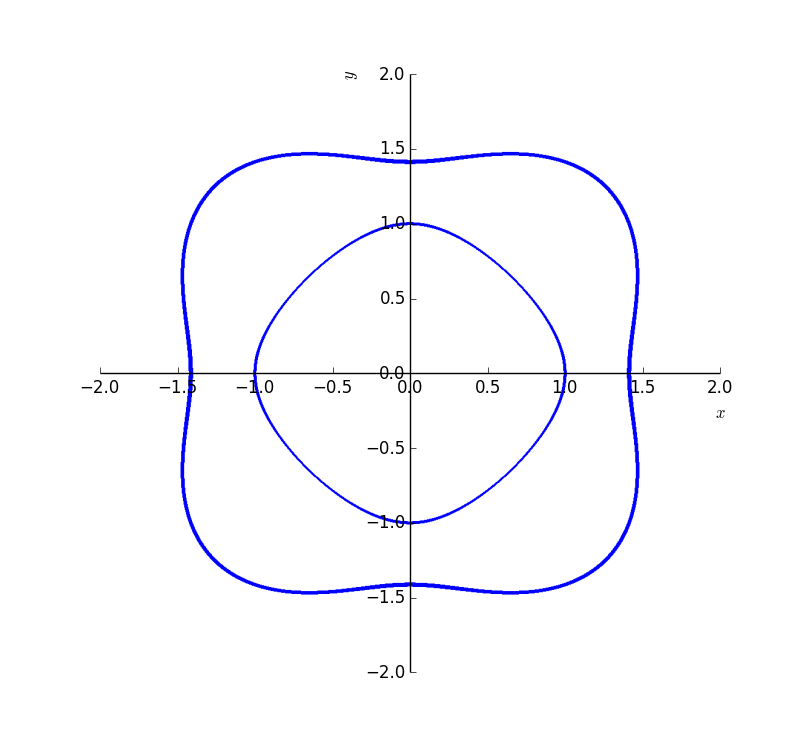
\includegraphics[width=0.7\textwidth]{images/helton-vinnikov.png}
  \caption{A real plot of the Helton-Vinnikov curve $f(x,y) = x^{4} +
    x^{2} y^{2} - 3 x^{2} + y^{4} - 3 y^{2} + 2$. The region bounded by
    the innermost oval is a spectrahedron.}
  \label{fig: spectrahedron}
\end{figure}

In some applications, it is important to have the matrices $A,B,C$ be
real when the curve $F$ is real. The representations important to
studying spectrahedra also require that the linear matrix represntation
is a {\it real definite representation}; that is, that the span of
$A,B,$ and $C$ contain a real positive definite matrix. Plaumann,
Sturmfels, and Vinzant \cite{PSV10} study several approaches to
computing real definite matrices of Helton--Vinnikov curves.

One approach, in fact the one chosen by Helton and Vinnikov, gives a
positive definite linear matrix representation of a Helton-Vinnikov
curve in terms of theta functions and the Schottky--Klein prime form.

\begin{theorem}
{\bf (Helton--Vinnikov)} Let $C : f(x,y,z) = 0$ be a real homogenous
curve of degree $d$ with $f(1,0,0) = 0$ and assume
\begin{enumerate}
  \item $C$ is a Helton--Vinnikov curve with the point $f(1,0,0) = 0$
    inside the innermost oval,
  \item the $d$ real intersection points with the line $\{z = 0\}$ are
    distinct non-singular points $Q_1,\ldots,Q_d$ with coordinates $Q_i
    = (-\beta_i : 1 : 0), \beta_i \neq 0$,
  \item $\delta$ is an even theta characteristic with
    $\theta[\delta](0,\Omega) \neq 0$.
\end{enumerate}
Then,
\[
    f(x,y,z) = \det \left( I_{d \times d}x + By + Cz \right)
\]
where $B = \text{diag}(\beta_1,\ldots,\beta_d)$, $C$ is a real
symmetric matrix with diagonal entries
\[
    c_{ii} = \beta_i
    \frac{\partial_z f(-\beta_i,1,0)}{\partial_y f(-\beta_i,1,0)},
\]
and off-diagonal entries
\[
    c_{jk} = \frac{\beta_k - \beta_j}{\theta[\delta](0,\Omega)}
    \frac{\theta[\delta](A(Q_k) - A(Q_j))}{E(Q_j,Q_k)},
\]
where $E : C \times C \to \CC^g$ is the Schottky--Klein prime form.
\end{theorem}

The calculation of linear matrix representations of Helton--Vinnikov
curves is an excellent application of the Schottky--Klein prime form and
I would like to provide an algorithm for doing so.
